\chapter{Symbolic Perturbation for {\tt insphere} Test}

This chapter describes a simple symbolic perturbation method for the {\tt insphere} test, so that we can assume there are no five points in $\mathbb{R}^3$ share a common circumscribed sphere. 

\section{The {\tt insphere} Test}

Let ${\bf a}, {\bf b}, {\bf c}, {\bf d}$ be four non-coplanar points in $\mathbb{R}^3$ and ${\bf e} \in \mathbb{R}^3$ be a fifth point.% and they form a positive orientation, i.e., $a, b, c$ follow the fingers of your left-hand's fist with thumb pointing to $d$. 
Let $\Sigma$ be the unique circumscribed sphere passing through the four points. The {\tt insphere} test is defined as follows
\begin{equation}
  \textrm{insphere}({\bf a}, {\bf b}, {\bf c}, {\bf d}, {\bf e})
  \left\{
  \begin{array}{ccl}
  > & 0, & \textrm{if ${\bf e}$ lies inside $\Sigma$},\\
  = & 0, & \textrm{if ${\bf e}$ lies on $\Sigma$},\\
  < & 0, & \textrm{if ${\bf e}$ lies outside $\Sigma$}.  
  \end{array}
  \right.
\end{equation}
It is well known that such test can be computed in the following way:
\begin{equation}\label{equ:insph}
 \textrm{insphere}({\bf a}, {\bf b}, {\bf c}, {\bf d}, {\bf e}) = \textrm{sign}\left(\frac{\textrm{det}({\bf A})}{\textrm{det}({\bf B})}\right).
\end{equation}
where ${\bf A}$ and ${\bf B}$ are two square matrices given below, $\textrm{det}()$ is the determinant function, and $\textrm{sign}(x)$ is the sign function, i.e., it returns one of $\{1, 0, -1\}$ depending on $x$ is large than, equal, or less than $0$, respectively.
\begin{equation}
  {\bf A} = \left[\begin{array}{ccccc}
      a_x & a_y & a_z & a_l & 1\\
      b_x & b_y & b_z & b_l & 1\\
      c_x & c_y & c_z & c_l & 1\\
      d_x & d_y & d_z & d_l & 1\\
      e_x & e_y & e_z & e_l & 1 
      \end{array}\right],
      \quad
  {\bf B} = \left[\begin{array}{cccc}
      a_x & a_y & a_z & 1\\
      b_x & b_y & b_z  & 1\\
      c_x & c_y & c_z  & 1\\
      d_x & d_y & d_z  & 1
      \end{array}\right].
\end{equation}
In the above, $a_l$ is obtained from the coordinates of $a$ by,
$a_l = a_x^2 + a_y^2 + a_z^2$.  The same for $b_l$, $c_l$, and $d_l$.

The $\textrm{insphere}$ test in $\mathbb{R}^3$ can be seen as an orientation test in $\mathbb{R}^4$ if there is a {\it lifting map} $\omega: \mathbb{R}^3 \to \mathbb{R}^4$ such that for each point ${\bf s} = (s_x, s_y, s_z)$ of $\mathbb{R}^3$ $\omega({\bf s}) = (s_x, s_y, s_z, s_l)$ of $\mathbb{R}^4$ with $s_l = s_x^2 + s_y^2 + s_z^2$.

\section{Symbolic Perturbation}

Five points in $\mathbb{R}^3$ have a common circumscribed sphere if and only if their images by $\omega$ lie in a hypeplane of $\mathbb{R}^4$. The symbolic perturbation of the {\tt insphere} test consists in adding respectively some value to the fourth coordinate of $\omega({\bf a}), \omega({\bf b}), \omega({\bf c}), \omega({\bf d}), \omega({\bf e})$ so that these points are not in the same hyperplane any more in $\mathbb{R}^4$. Then the predicate answers positive or negative instead of zero.

Let $S$ be a finite set of $n$ points be ordered like $\{{\bf s}_1, {\bf s}_2, {\bf s}_3, ... {\bf s}_{n}\}$ in $\mathbb{R}^3$. For each point ${\bf s} \in S$, we perturb it by adding a perturbation in $\omega({\bf s})$ by
\begin{equation}
\omega({\bf s}) = (s_{x}, s_{y}, s_{z}, s_{l}-s_{w}),
\end{equation}
where $s_w$ is an infinitesimal and $s_w > 0$. The quantity of the perturbation will determine the final result of the {\tt insphere} test. We will discuss it at the end of this section.

Now assume ${\bf a}, {\bf b}, {\bf c}, {\bf d}, {\bf e}$ lie on a common circumscribed sphere, i.e., $\textrm{det}({\bf A}) = 0$. We re-compute the {\tt insphere} test by using the five perturbed points $\omega({\bf a}), \omega({\bf b}), \omega({\bf c}), \omega({\bf d}), \omega({\bf e})$, i.e., 
\[
  \textrm{insphere}(\omega({\bf a}), \omega({\bf b}), \omega({\bf c}), \omega({\bf d}), \omega({\bf e})) = \textrm{sign}\left(\frac{\textrm{det}({\bf A}^{\omega})}{\textrm{det}({\bf B})}\right)
\]
Where
\begin{equation}
  {\bf A}^{\omega} = \left[\begin{array}{ccccc}
      a_x & a_y & a_z & a_l - a_w & 1\\
      b_x & b_y & b_z & b_l - b_w & 1\\
      c_x & c_y & c_z & c_l - c_w & 1\\
      d_x & d_y & d_z & d_l - d_w & 1\\
      e_x & e_y & e_z & e_l - e_w & 1 
      \end{array}\right].
\end{equation}

Since the determinant is a linear function and by the assumption that ${\bf a}$, ${\bf b}$, ${\bf c}$, ${\bf d}$, and ${\bf e}$ are co-spherical. We can compute $\textrm{det}({\bf A}^{\omega})$ by
\[
  \begin{array}{rcl}
  \textrm{det}({\bf A}^{\omega}) &=& \textrm{det}\left(
      \left[\begin{array}{ccccc}
      a_x & a_y & a_z & a_l & 1\\
      b_x & b_y & b_z & b_l & 1\\
      c_x & c_y & c_z & c_l & 1\\
      d_x & d_y & d_z & d_l & 1\\
      e_x & e_y & e_z & e_l & 1 
      \end{array}\right]\right)
    + \textrm{det}\left(
      \left[\begin{array}{ccccc}
      a_x & a_y & a_z & 1 & a_w\\
      b_x & b_y & b_z & 1 & b_w\\
      c_x & c_y & c_z & 1 & c_w\\
      d_x & d_y & d_z & 1 & d_w\\
      e_x & e_y & e_z & 1 & e_w
      \end{array}\right]\right)\\
    &=& \textrm{det}\left(
      \left[\begin{array}{ccccc}
      a_x & a_y & a_z & 1 & a_w\\
      b_x & b_y & b_z & 1 & b_w\\
      c_x & c_y & c_z & 1 & c_w\\
      d_x & d_y & d_z & 1 & d_w\\
      e_x & e_y & e_z & 1 & e_w
      \end{array}\right]\right).\\
  \end{array}
\]
Expand the above determinant along the last column\footnote{The determinant formula
\[
  \textrm{det}({\bf A}) = \sum_{j=1}^{n} (-1)^{i+j} a_{ij} {\bf M}_{ij}({\bf A}),
\]
where ${\bf A}$ is a $n \times n$ matrix, ${\bf M}_{ij}(a)$ (called the {\it $(i,j)$ minor} of $a$) is the determinant of the $(n-1) \times (n-1)$ submatrix of ${\bf A}$ formed by deleting $i$-th row and $j$-th column of $a$.}, we get
\begin{equation}\label{equ:perturb}
  \textrm{det}({\bf A}^{\omega}) = a_w \textrm{det}({\bf A}_a) - b_w \textrm{det}({\bf A}_b) + c_w \textrm{det}({\bf A}_c) - d_w \textrm{det}({\bf A}_d) + e_w \textrm{det}({\bf A}_e).
\end{equation}
where
\[
  \begin{array}{ccccc}
  \textrm{det}({\bf A}_a) &=& \textrm{det}\left(\left[\begin{array}{cccc}
              b_x & b_y & b_z & 1\\
              c_x & c_y & c_z & 1\\
              d_x & d_y & d_z & 1\\
              e_x & e_y & e_z & 1 
              \end{array}\right]\right) 
              &=& \textrm{orient3d}({\bf b}, {\bf c}, {\bf d}, {\bf e});\\ 
   \textrm{det}({\bf A}_b) &=& \textrm{det}\left(\left[\begin{array}{cccc}
               a_x & a_y & a_z & 1\\
               c_x & c_y & c_z & 1\\
               d_x & d_y & d_z & 1\\
               e_x & e_y & e_z & 1 
               \end{array}\right]\right)
              &=& \textrm{orient3d}({\bf a}, {\bf c}, {\bf d}, {\bf e});\\
    \textrm{det}({\bf A}_c) &=& \textrm{det}\left(\left[\begin{array}{cccc}
                a_x & a_y & a_z & 1\\
                b_x & b_y & b_z & 1\\
                d_x & d_y & d_z & 1\\
                e_x & e_y & e_z & 1 
                \end{array}\right]\right)
               &=& \textrm{orient3d}({\bf a}, {\bf b}, {\bf d}, {\bf e});\\ 
     \textrm{det}({\bf A}_d) &=& \textrm{det}\left(\left[\begin{array}{cccc}
                 a_x & a_y & a_z & 1\\
                 b_x & b_y & b_z & 1\\
                 c_x & c_y & c_z & 1\\
                 e_x & e_y & e_z & 1 
                 \end{array}\right]\right)
               &=& \textrm{orient3d}({\bf a}, {\bf b}, {\bf c}, {\bf e});\\
      \textrm{det}({\bf A}_e) &=& \textrm{det}\left(\left[\begin{array}{cccc}
                  a_x & a_y & a_z & 1\\
                  b_x & b_y & b_z & 1\\
                  c_x & c_y & c_z & 1\\
                  d_x & d_y & d_z & 1
                  \end{array}\right]\right)
               &=& \textrm{orient3d}({\bf a}, {\bf b}, {\bf c}, {\bf d}).
  \end{array}
\]

Since we assume that the four points ${\bf a}$, ${\bf b}$, ${\bf c}$, and ${\bf d}$ are non-coplanar, hence $\textrm{det}({\bf A}_e) \neq 0$. Moreover, this assumption implies that there are at most one determinant in $\textrm{det}({\bf A}_a), ..., \textrm{det}({\bf A}_d)$ can be zero, otherwise, ${\bf a}$, ${\bf b}$, ${\bf c}$, and ${\bf d}$ would be coplanar. It is possible to let $\textrm{det}({\bf A}^{\omega})$ not be zero by appropriate choosing the perturbations $a_w, ..., e_w$.

A simple strategy is to choose such a perturbations i to let $a_w >> b_w >> c_w >> d_w >> e_w$. Then the sign of $\textrm{det}({\bf A}^{\omega})$ is determined by the first non-zero determinant in the right hand side of (\ref{equ:perturb}). 

One way to implement the above strategy is to use the index of the points, i.e., {\it the one with smaller index gets bigger perturbation than the one with higher index}.

\section{Examples}

This section gives few examples to illustrate how the perturbation technique of the above section work.  In the following examples, let ${\bf a}, {\bf b}, {\bf c}, {\bf d}, {\bf e}$ are points in $\mathbb{R}^3$ and their indices are in increasing order.

\begin{figure}
\centering{
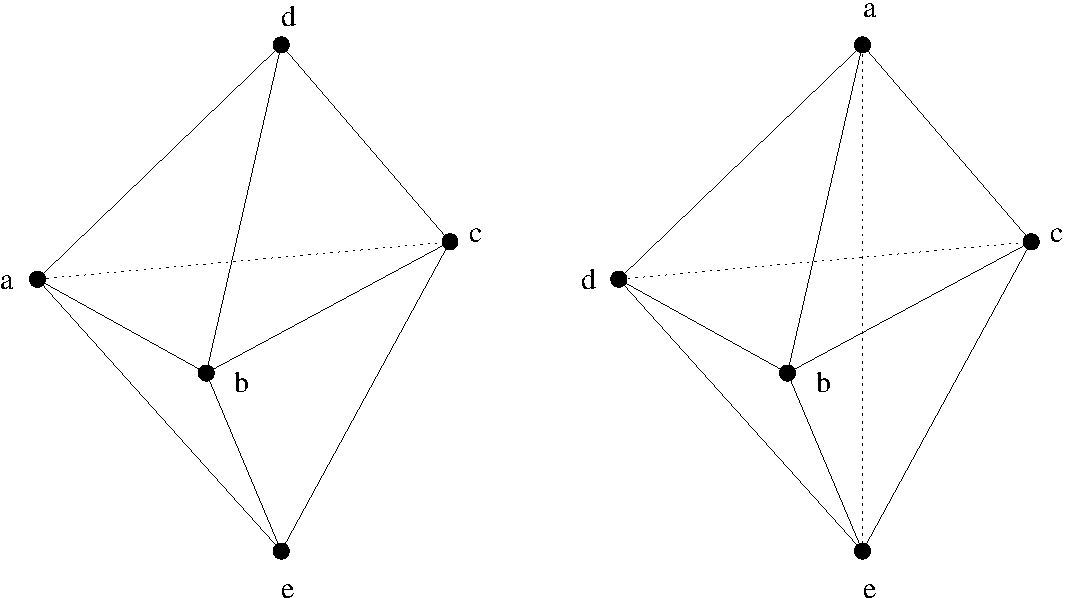
\includegraphics[width=0.8\textwidth]{../figs/symbolicperturb1}
}
\caption{Symbolic perturbation. The five points ${\bf a}, {\bf b}, {\bf c}, {\bf d}, {\bf e}$ share a circumscribed sphere.}
\label{fig:ex1}
\end{figure}

The first example (see Figure~\ref{fig:ex1}) is in the case which no four points are coplanar. The two pictures show the same five points but the labeling of points are different.  In the left figure, let's evaluate
\[
\begin{array}{rcl}
\textrm{insphere}({\bf a}, {\bf b}, {\bf c}, {\bf e}, {\bf d}) &=&
a_w\textrm{orient3d}({\bf b}, {\bf c}, {\bf e}, {\bf d})\\
& & -b_w\textrm{orient3d}({\bf a}, {\bf c}, {\bf e}, {\bf d})\\
& & +c_w\textrm{orient3d}({\bf a}, {\bf b}, {\bf e}, {\bf d})\\
& & -e_w\textrm{orient3d}({\bf a}, {\bf b}, {\bf c}, {\bf d})\\
& & +d_w\textrm{orient3d}({\bf a}, {\bf b}, {\bf c}, {\bf e})\\
&\approx& a_w\textrm{orient3d}({\bf b}, {\bf c}, {\bf e}, {\bf d})\\
&<& 0
\end{array}
\]
and
\[
\begin{array}{rcl}
\textrm{insphere}({\bf e}, {\bf d}, {\bf b}, {\bf a}, {\bf c}) &=&
e_w\textrm{orient3d}({\bf d}, {\bf b}, {\bf a}, {\bf c})\\
& & -d_w\textrm{orient3d}({\bf e}, {\bf b}, {\bf a}, {\bf c})\\
& & +b_w\textrm{orient3d}({\bf e}, {\bf d}, {\bf a}, {\bf c})\\
& & -a_w\textrm{orient3d}({\bf e}, {\bf d}, {\bf b}, {\bf c})\\
& & +c_w\textrm{orient3d}({\bf e}, {\bf d}, {\bf b}, {\bf a})\\
&\approx& -a_w\textrm{orient3d}({\bf e}, {\bf d}, {\bf b}, {\bf c})\\
&>& 0  \quad \textrm{(non-Delaunay)}
\end{array}
\]

The tests show that tetrahedra ${\bf abcd}$ and ${\bf bace}$ are Delaunay.  While ${\bf edab}$, ${\bf edbc}$, and ${\bf edca}$ are not, which are consistent.

In the right figure, let's evaluate 
\[
\begin{array}{rcl}
\textrm{insphere}({\bf d}, {\bf b}, {\bf c}, {\bf e}, {\bf a}) &=&
d_w\textrm{orient3d}({\bf b}, {\bf c}, {\bf e}, {\bf a})\\
& & -b_w\textrm{orient3d}({\bf d}, {\bf c}, {\bf e}, {\bf a})\\
& & +c_w\textrm{orient3d}({\bf d}, {\bf b}, {\bf e}, {\bf a})\\
& & -e_w\textrm{orient3d}({\bf d}, {\bf b}, {\bf c}, {\bf a})\\
& & +a_w\textrm{orient3d}({\bf d}, {\bf b}, {\bf c}, {\bf e})\\
&\approx& a_w\textrm{orient3d}({\bf d}, {\bf b}, {\bf c}, {\bf e})\\
&>& 0 \quad \textrm{(non-Delaunay)}
\end{array}
\]
and
\[
\begin{array}{rcl}
\textrm{insphere}({\bf e}, {\bf a}, {\bf b}, {\bf d}, {\bf c}) &=&
e_w\textrm{orient3d}({\bf a}, {\bf b}, {\bf d}, {\bf c})\\
& & -a_w\textrm{orient3d}({\bf e}, {\bf b}, {\bf d}, {\bf c})\\
& & +b_w\textrm{orient3d}({\bf e}, {\bf a}, {\bf d}, {\bf c})\\
& & -d_w\textrm{orient3d}({\bf e}, {\bf a}, {\bf b}, {\bf c})\\
& & +c_w\textrm{orient3d}({\bf e}, {\bf a}, {\bf b}, {\bf d})\\
&\approx& -a_w\textrm{orient3d}({\bf e}, {\bf b}, {\bf d}, {\bf c})\\
&<& 0
\end{array}
\]
The tests are consistent.

\begin{figure}
\centering{
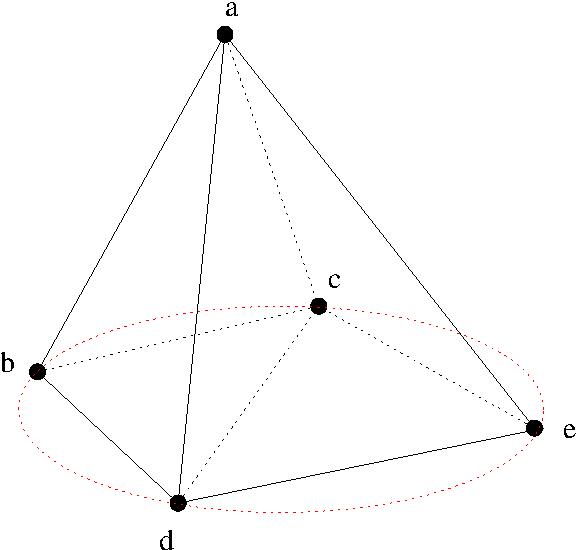
\includegraphics[width=0.4\textwidth]{../figs/symbolicperturb2}
}
\caption{Symbolic perturbation of five coplanar points. In this example, four point are coplanar.}
\label{fig:ex2}
\end{figure}

The second example (see Fig.~\ref{fig:ex2}) illustrates the case which four points ${\bf b}, {\bf c}, {\bf d}, {\bf e}$ are coplanar and cospherical. Let's evaluate 
\[
\begin{array}{rcl}
\textrm{insphere}({\bf d},{\bf c},{\bf a},{\bf b},{\bf e}) &=&
d_w\textrm{orient3d}({\bf c},{\bf a},{\bf b},{\bf e})\\
& & -c_w\textrm{orient3d}({\bf d},{\bf a},{\bf b},{\bf e})\\
& & +a_w\textrm{orient3d}({\bf d},{\bf c},{\bf b},{\bf e})\\
& & -b_w\textrm{orient3d}({\bf d},{\bf c},{\bf a},{\bf e})\\
& & +e_w\textrm{orient3d}({\bf d},{\bf c},{\bf a},{\bf b})\\
&\approx& +a_w\textrm{orient3d}({\bf d},{\bf c},{\bf b},{\bf e})\\
& & -b_w\textrm{orient3d}({\bf d},{\bf c},{\bf a},{\bf e})\\
&>& 0  \quad \textrm{(non-Delaunay)}
\end{array}
\]
and
\[
\begin{array}{rcl}
\textrm{insphere}({\bf b},{\bf e},{\bf a},{\bf c},{\bf d}) &=&
b_w\textrm{orient3d}({\bf e},{\bf a},{\bf c},{\bf d})\\
& & -e_w\textrm{orient3d}({\bf b},{\bf a},{\bf c},{\bf d})\\
& & +a_w\textrm{orient3d}({\bf b},{\bf e},{\bf c},{\bf d})\\
& & -c_w\textrm{orient3d}({\bf b},{\bf e},{\bf a},{\bf d})\\
& & +d_w\textrm{orient3d}({\bf b},{\bf e},{\bf a},{\bf c})\\
&\approx& +a_w\textrm{orient3d}({\bf b},{\bf e},{\bf c},{\bf d})\\
& & +b_w\textrm{orient3d}({\bf e},{\bf a},{\bf c},{\bf d})\\
&<& 0
\end{array}
\]
The tests show that the two tetrahedra containing edge ${\bf cd}$ are non-Delaunay, while the two containing edge ${\bf be}$ are Delaunay, which are consistent.